\documentclass[12pt]{ctexart}
    \title{PING程序的实现}
    \author{162020321 朱家震}
    \pagestyle{empty}
    \usepackage{amsmath}
    \usepackage[a4paper,left=2.5cm,right=2.5cm,top=2cm,bottom=2cm]{geometry}
    \usepackage{amsfonts}
    \usepackage{amssymb}
    \usepackage{amsthm,amsmath}
    \usepackage{mathrsfs}
    \usepackage{indentfirst}
    \usepackage{multirow}
    \usepackage{graphicx}
    \usepackage{float}
    %\usepackage{pythonhighlight}
    \usepackage{subfigure}
    \usepackage[usenames,dvipsnames]{xcolor}
    \usepackage[ruled,linesnumbered]{algorithm2e}
    \usepackage{bm} 
    \usepackage{listings}
    \newfontfamily\courier{Courier New}
    \lstset{linewidth=1.1\textwidth,
            numbers=left, %设置行号位置 
            basicstyle=\small\courier,
            numberstyle=\tiny\courier, %设置行号大小  
            keywordstyle=\color{blue}\courier, %设置关键字颜色  
            %identifierstyle=\bf,
            commentstyle=\it\color[cmyk]{1,0,1,0}\courier, %设置注释颜色 
            stringstyle=\it\color[RGB]{128,0,0}\courier,
            %framexleftmargin=10mm,
            frame=single, %设置边框格式  
            backgroundcolor=\color[RGB]{245,245,244},
            %escapeinside=``, %逃逸字符(1左面的键),用于显示中文  
            breaklines, %自动折行  
            extendedchars=false, %解决代码跨页时,章节标题,页眉等汉字不显示的问题  
            xleftmargin=0em,xrightmargin=2em, aboveskip=1em, %设置边距  
            tabsize=4, %设置tab空格数  
            showspaces=false %不显示空格  
            basicstyle=\small\courier
           }  
\makeatletter %使\section中的内容左对齐
%\renewcommand{\section}{\@startsection{section}{1}{0mm}
% {-\baselineskip}{0.5\baselineskip}{\bf\leftline}}
\makeatother
%\renewcommand\thesubsectiondis{\section.\arabic{subsection}}  %重定义语句
\begin{document}
    \maketitle
    \setcounter{section}{0}
    \section{实验内容}
    \subsection{实验目的}

    理解ping程序的概念,熟练使用原始套接字

    \subsection{实验环境}

    Linux,C

    \subsection{实验内容}

    \begin{enumerate}
        \item 设计一个简单的PING程序,每隔1秒钟使用ICMP报文向目的IP地址发一个ICMP请求(长度由length指定),对方将返回一个ICMP应答,应答数据包通过循环调用函数recvfrom来接收。发送ICMP报文的次数由counts指定
        \item ping dstIP –l length –n counts
    \end{enumerate}
    
    \section{实验设计}
    \subsection{ping程序执行}

    首先我们执行ping程序,了解我们要做的输出是什么样的,执行出来的效果如下:
    
    \begin{figure}[H]
        \centering
        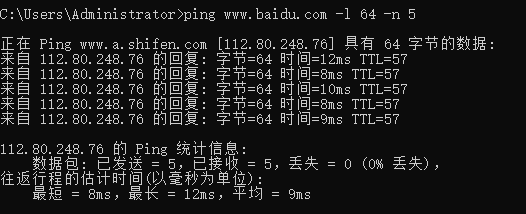
\includegraphics[width=5in]{figures/win.png}
        \label{sw}
        \caption{windows终端执行结果}
    \end{figure}

    \begin{figure}[H]
        \centering
        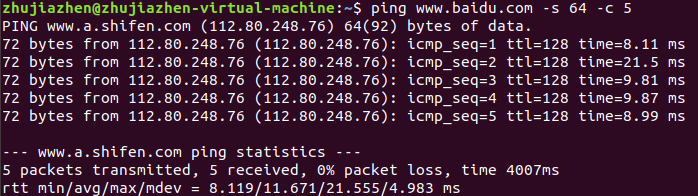
\includegraphics[width=5in]{figures/linux.png}
        \label{li}
        \caption{Linux终端执行结果}
    \end{figure}

    我们接下来就根据Linux的输出结果进行一个复现。

    \subsection{程序分块}

    根据题意,我们可以将代码分为几个重要部分:计算校验和、发送ICMP请求
    以及接受ICMP请求。各个函数的具体实现在下一部分讲解。

    \section{关键程序}
    \subsection{计算校验和}

    \begin{flushleft}
    \begin{lstlisting}[language = C]
unsigned short calcChecksum(unsigned short *addr, int len)
{
    unsigned int sum = 0;
    unsigned short answer = 0;
    unsigned short *w = addr;
    int nleft = len;

    while (nleft > 1) {
        sum += *w++;
        nleft -= 2;
    }

    if (nleft == 1) {
        *(unsigned char *)(&answer) = *(unsigned char *)w;
        sum += answer;
    }

    sum = (sum >> 16) + (sum & 0xFFFF);
    sum += (sum >> 16);
    answer = ~sum;
    return answer;
}
    \end{lstlisting}
\end{flushleft}

    校验和是为了确保数据在传输过程中的完整性。接收方可以通过校验和验证数据是否被篡改或损坏。

    `calcChecksum`函数使用了标准的互联网校验和算法,对每个16位的字进行求和,并进行溢出的处理。
    同时,计算校验和时使用无符号短整型(unsigned short)是为了确保计算的结果符合互联网校验和算法的规范。
    如果使用有符号短整型(short),可能会导致计算结果出现溢出或不符合预期,因为有符号短整型的范围是从负数到正数,而不是从0到正数。

    \subsection{发送ICMP请求}

    \begin{lstlisting}[language = C]
int sendPingRequest(int sockfd, struct sockaddr_in *dest_addr, int packet_size, int seq)
{
    struct icmp *icmp_packet;
    char send_packet[PACKET_SIZE];
    int packet_len;

    icmp_packet = (struct icmp *)send_packet;
    icmp_packet->icmp_type = ICMP_ECHO;
    icmp_packet->icmp_code = 0; // 询问报文  
    icmp_packet->icmp_id = getpid();
    icmp_packet->icmp_seq = seq;
    memset(icmp_packet->icmp_data, 0xa5, packet_size);
    gettimeofday((struct timeval *)icmp_packet->icmp_data, NULL);

    packet_len = 8 + packet_size;
    icmp_packet->icmp_cksum = 0;
    icmp_packet->icmp_cksum = calcChecksum((unsigned short *)icmp_packet, packet_len);

    if (sendto(sockfd, send_packet, packet_len, 0, 
        (struct sockaddr *)dest_addr, sizeof(struct sockaddr)) == -1) {
        perror("sendto error");
        return -1;
    }

    return 0;
}        
    \end{lstlisting}

    发送函数中,我们使用了icmp结构体:
    \begin{lstlisting}[language = C]
struct icmphdr {
    uint8_t type;        // ICMP 报文类型
    uint8_t code;        // ICMP 报文代码
    uint16_t checksum;   // ICMP 报文校验和
    // 其他字段根据不同的 ICMP 报文类型可以有不同的定义
};
\end{lstlisting}

    数据部分被填充为0xa5,并使用`memset`函数将数据部分的字节设置为指定的值。这是为了在发送方和接收方之间提供一致的数据,以便检查传输的正确性。

    \subsection{接收ICMP请求}

    \begin{lstlisting}[language = C]
int receivePingResponse(int sockfd, int seq)
{
    char recv_packet[PACKET_SIZE];
    struct sockaddr_in from;
    socklen_t from_len;
    int packet_len;

    while (1) {
        memset(recv_packet, 0, sizeof(recv_packet));
        from_len = sizeof(from);

        if ((packet_len = recvfrom(sockfd, recv_packet, sizeof(recv_packet), 0, 
                    (struct sockaddr *)&from, &from_len)) == -1) {
            perror("recvfrom error");
            return -1;
        }
        // printf("Received ICMP response from: %s\n", inet_ntoa(from.sin_addr));

        // 解析ICMP应答
        struct ip *ip_packet = (struct ip *)recv_packet;
        struct icmp *icmp_packet = (struct icmp *)(recv_packet + (ip_packet->ip_hl << 2));

        if (icmp_packet->icmp_type == ICMP_ECHOREPLY && icmp_packet->icmp_id == getpid()
            && icmp_packet->icmp_seq == seq) {
        struct timeval *st = (struct timeval *)icmp_packet->icmp_data;
        struct timeval ct;
        gettimeofday(&ct, NULL);

        double rtt = (ct.tv_sec - st->tv_sec) * 1000.0 + (ct.tv_usec - st->tv_usec) / 1000.0;
            printf("%d bytes from %s: icmp_seq=%d time=%.2fms ttl=%d\n",
               packet_len, inet_ntoa(from.sin_addr), seq, rtt, ip_packet->ip_ttl);
        // printf("ICMP response received.\n");
            break;
        }
    }

    return 0;
}
    \end{lstlisting}

    在接受icmp函数中,
    首先,根据IP首部的长度字段找到ICMP首部的位置。
    然后,检查ICMP类型是否为ICMP回显应答,并验证ICMP标识和序列
    号与发送的请求是否匹配。最后,计算往返时间(RTT)并输出相关
    信息。

    \subsection{主函数}

    在主函数解析地址时,`inet\_pton`函数用于将点分十进制表示的IPv4地址转换为二进制形式。而`gethostbyname`函数用于解析主机名,将主机名转换为IP地址。

    \section{实验结果与分析}

    最后,myping的运行结果如下:

    \begin{figure}[H]
        \centering
        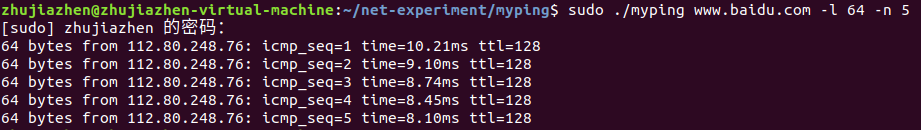
\includegraphics[width=5in]{figures/res.png}
        \label{rw}
        \caption{myping终端执行结果}
    \end{figure}

    可以看出结果较为清晰,比较真实的还原了Linux上ping的输出结果。

\end{document}